\documentclass[11pt]{beamer}
\usetheme{Montpellier}
\usefonttheme[onlymath]{serif}
\usecolortheme{rose}

\usepackage{tikz} \usepackage{graphicx} \usepackage{algorithm} \usepackage[noend]{algpseudocode} \usepackage{caption}
\usepackage{amsmath} \usepackage{pgfplots} \usepackage{float}

\usetikzlibrary{shapes.geometric, arrows}

\setbeamertemplate{navigation symbols}{}
\setbeamerfont{page number in head/foot}{size=\fontsize{9}{11}}
\setbeamertemplate{footline}[frame number]
\setbeamertemplate{section in toc}{\inserttocsectionnumber.~\inserttocsection}
\setbeameroption{show notes}  % Comment this out to not show the notes.

\author{Glenn Galvizo, under Dr. Floyd Reed}
\title{Efficient Parameter Estimation for Human Microsatellite Mutation}
\institute{University of Hawaii at Manoa}

% Has to be in the preamble...
\usetikzlibrary{calligraphy}

\begin{document}
    \begin{frame}
        \titlepage
    \end{frame}

	\section{Introduction}\label{sec:i}
	\begin{frame}
		\frametitle{Overview}
        \tableofcontents

        \note{
            \footnotesize
            \begin{enumerate}
                \item Introduce research, talk about human history.
                \item Talk about microsatellites, what they are and my mutation model.
                \item How to find the best parameters for my model.
                \item What the best parameters are.
            \end{enumerate}
        }
	\end{frame}

	\begin{frame}
		\frametitle{A brief overview of modern human history:}
        \centering{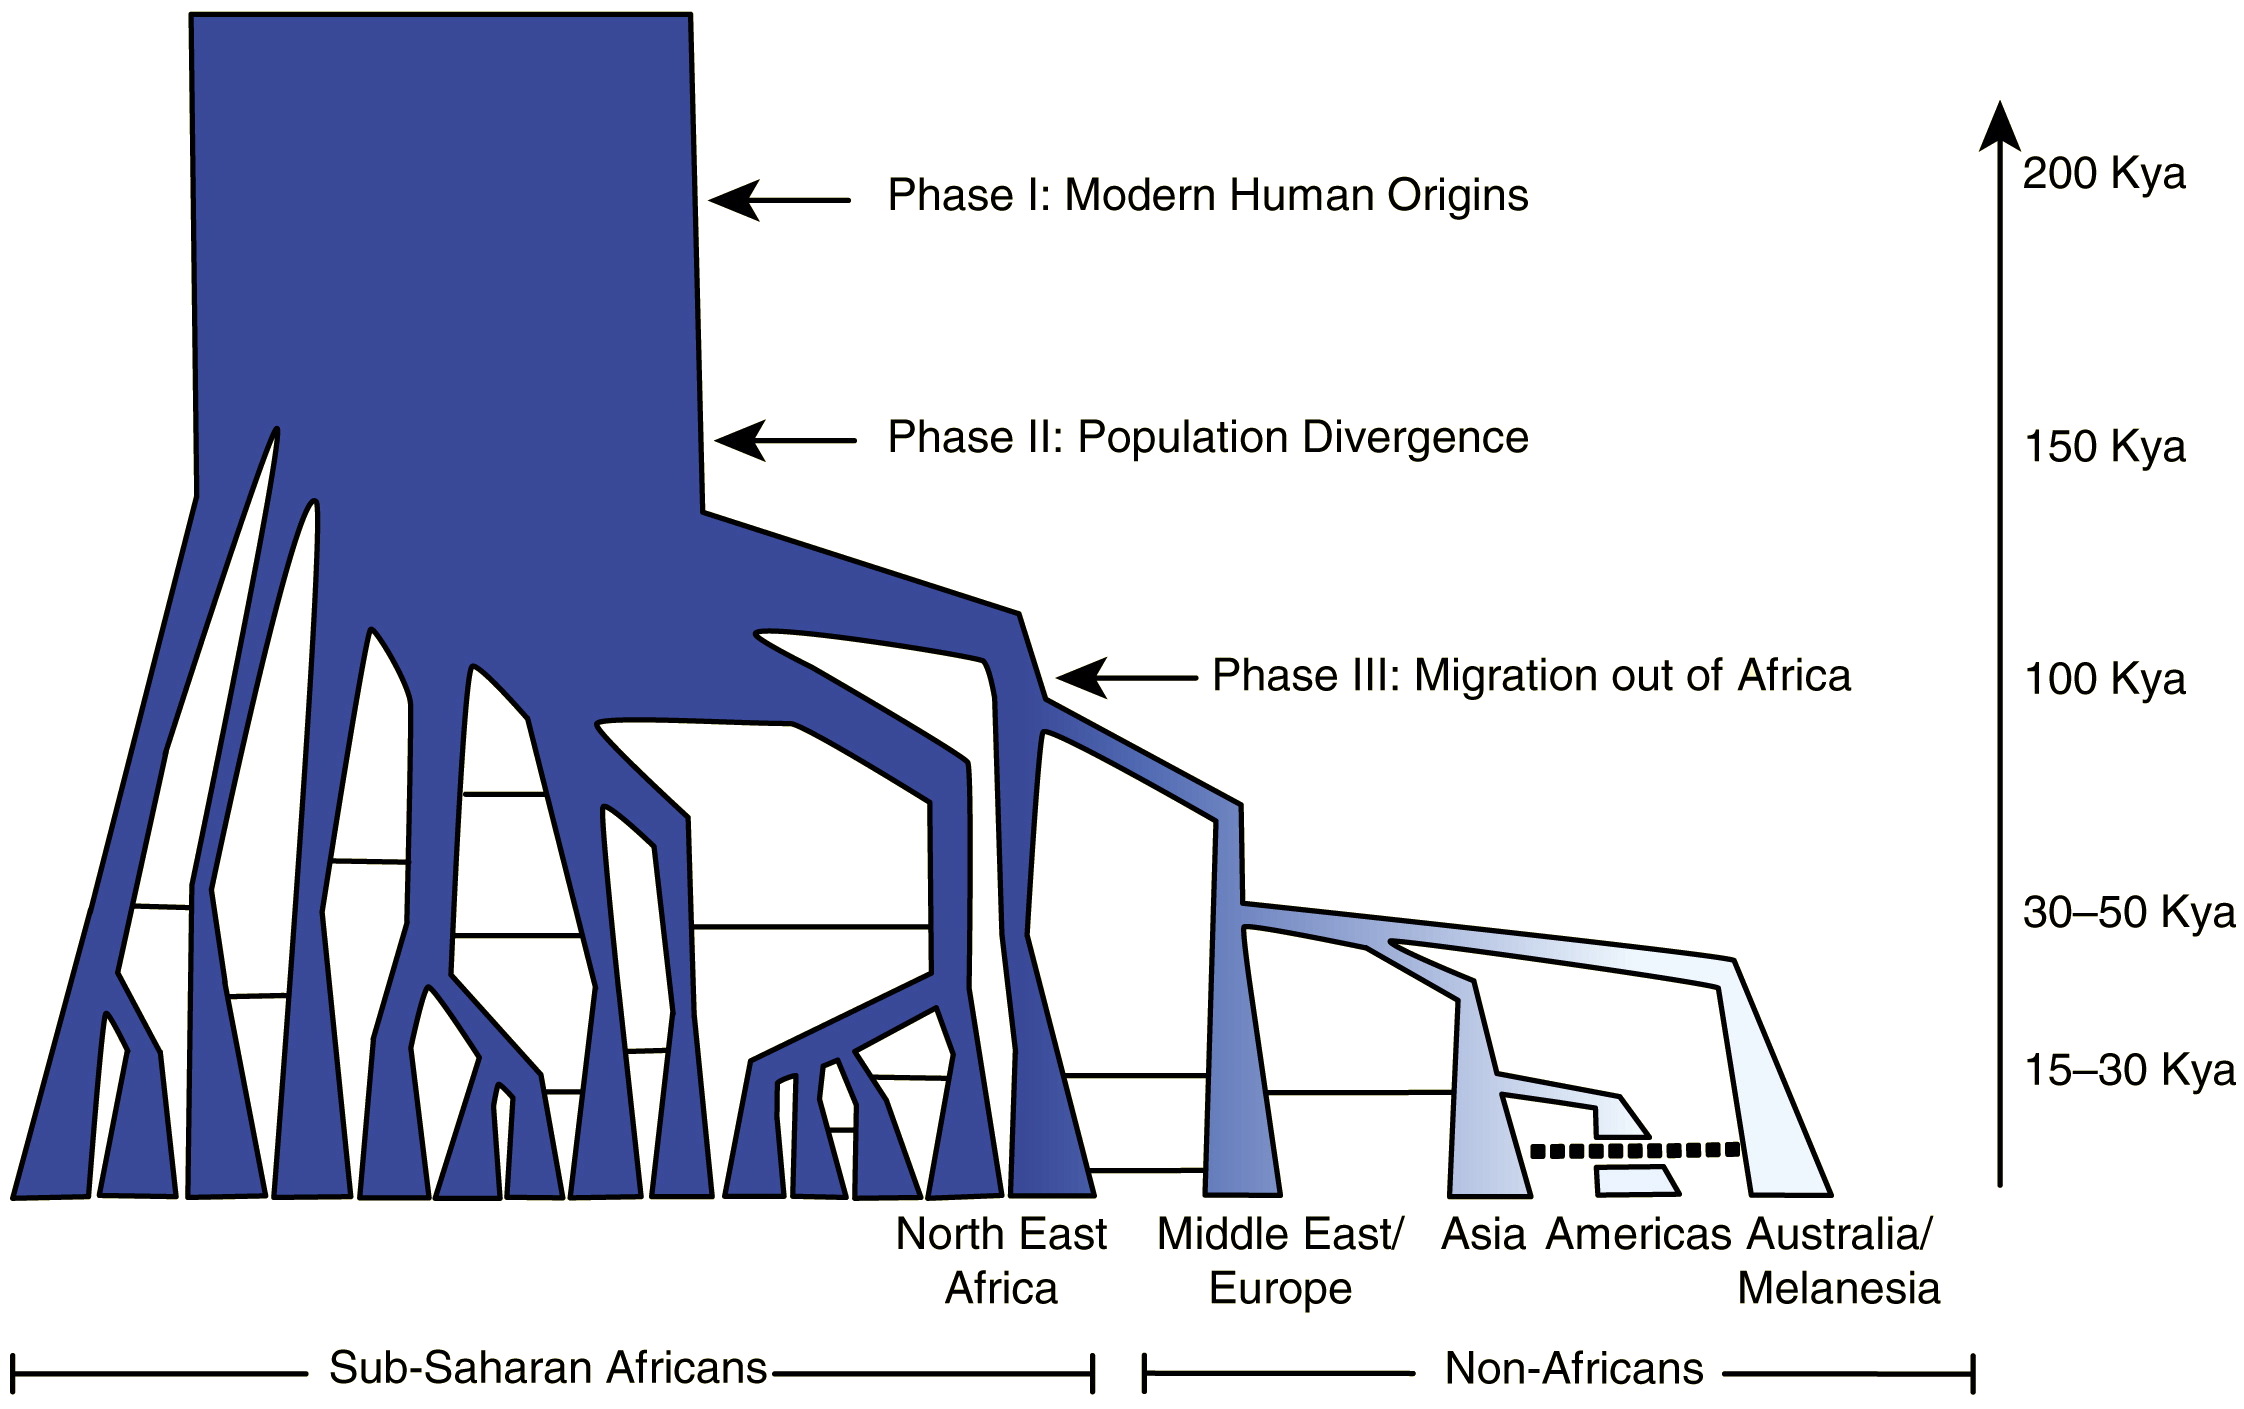
\includegraphics[scale=0.9]{images/modern-human-history.png}}

        \note{
            \footnotesize
            \begin{enumerate}
                \item Start with the origin of modern humans.
                \item What do we know about human history?
                \item We have some common ancestor in Africa.
                \item Graph, x axis is geographical location, y axis is time.
                \item Modern humans emerged 200,000 years ago.
                \item We migrated out of Africa 100,000 years ago to Europe and Middle East, then
                    Asia / America / Australia.
                \item How do we know this?- Variations in DNA!
                \item Basis of research: Explore different evolutionary models using highly variable genetic marker.
            \end{enumerate}
        }
	\end{frame}

	\subsection{Problem Statement}\label{subsec:ps}
	\begin{frame}
		\frametitle{What is the goal of this research?}
        \begin{block}{Problem Statement}
            \emph{Which microsatellite mutation model parameters most likely produce our observed data?}
        \end{block} \medskip

        \begin{block}{Essential Questions}
            \begin{enumerate}
                \item What is a microsatellite?
                \item What is the observed data?
                \item How do microsatellites mutate?
                    What is the model?
                \item How do we simulate evolution?
                \item How can we find the best parameters?
            \end{enumerate}
        \end{block}

        \note{
            \footnotesize
            \begin{enumerate}
                \item Verbatim, my problem statement is: \ldots
                \item Dissecting this, we get the following essential questions: \ldots
            \end{enumerate}
        }
	\end{frame}

	\section{Microsatellites}\label{sec:mi}
	\subsection{DNA Variation: Tandem Repeats}\label{subsec:dvtr}
    \begin{frame}
        \frametitle{What is a microsatellite?}
        \begin{definition}[Microsatellite]
            A \emph{microsatellite} is a short sequence in DNA, repeated in tandem.
        \end{definition} \bigskip

        \begin{columns}
            \begin{column}{0.4\textwidth}
                \begin{itemize}
                    \item Interested in number of repeats.
                    \item Represent variation in humans.
                    \item More variable than SNP marker~\cite{gemayelJunkVariableTandemRepeats2012}.
                \end{itemize}
            \end{column}
            \begin{column}{0.6\textwidth}
                \begin{equation*}
                    \begin{aligned}
                         \ldots &\text{AACG}\textbf{ATATATATATAT}\text{GGCTA} \ldots \\
                         \ldots &\text{AACG}\textbf{ATATATATAT}\text{GGCTA} \ldots \\
                         \ldots &\text{AACG}\textbf{ATATATAT}\text{GGCTA} \ldots \\
                         \ldots &\text{AACG}\textbf{ATATAT}\text{GGCTA} \ldots \\
                         \ldots &\text{AACG}\textbf{ATAT}\text{GGCTA} \ldots
                    \end{aligned}
                \end{equation*}
            \end{column}
        \end{columns}

        \note{
            \footnotesize
            \begin{enumerate}
                \item Let's start with the first essential question: \ldots
                \item Form of genetic variation in which short sequences of DNA are repeated in tandem.
                \item Variation = how many times this short sequence is repeated.
                \item On the right, five microsatellite variants with AT as the repeated sequence.
                \item One individual in a population can have the variant on top, with 5 repeats of AT.
                    Another individual can have the variant on the bottom, with 2 repeats of AT.
                \item Infer human history by tracking the changes in repeat length over generations.
                \item A more popular marker for genetic variation is the SNP, but we use microsatellites because they
                    mutate more often.
                    More mutations means that we can potentially infer more in a shorter time period.
            \end{enumerate}
        }
    \end{frame}

    \subsection{Microsatellite Data}\label{subsec:md}
    \begin{frame}
        \frametitle{What data are we working with?} \bigskip
        \centering{\pgfplotsset{compat=1.5}
\usetikzlibrary{pgfplots.groupplots}
\pgfmathdeclarefunction{gauss}{2}{%
  \pgfmathparse{1/(#2*sqrt(2*pi))*exp(-((x-#1)^2)/(2*#2^2))}%
}

\begin{tikzpicture}
    \begin{groupplot}[
        group style={
        group name=my plots,
        group size=3 by 3,
        vertical sep=0pt,
        horizontal sep=2pt,
        ylabels at=edge left,
        xlabels at=edge bottom,
    },
    ticks=none, xmin=0, xmax=10,
    domain=0:10, samples=25,
%    xlabel={Repeat Unit},
%    ylabel={Frequency},
    width=0.44\linewidth, height=3cm]
        \nextgroupplot
        \addplot [very thick,blue!50!black] {gauss(4,1)};
        \nextgroupplot
        \addplot [very thick,blue!50!black] {gauss(3,7)};
        \nextgroupplot
        \addplot [very thick,blue!50!black] {gauss(7,2)};
        \nextgroupplot[ylabel=Frequency]
        \addplot [very thick,blue!50!black] {gauss(2,0.5)};
        \nextgroupplot
        \addplot [very thick,blue!50!black] {gauss(5,1)};
        \nextgroupplot
        \addplot [very thick,blue!50!black] {gauss(3,0.3)};
        \nextgroupplot
        \addplot [very thick,blue!50!black] {gauss(1,1)};
        \nextgroupplot[xlabel=Repeat Unit]
        \addplot [very thick,blue!50!black] {gauss(2,2.5)};
        \nextgroupplot
        \addplot [very thick,blue!50!black] {gauss(8,8)};
    \end{groupplot}
\end{tikzpicture}}
        \bigskip
        \newline
        \centering{\emph{Populations of \text{GATA} microsatellite variations, interested in frequency of a
        repeat length.}}

        \note{
            \footnotesize
            \begin{enumerate}
                \item Next essential question, \ldots
                \item The data we are working with = observed populations of microsatellites variants.
                \item These variants have GATA as their repeat sequence.
                \item Interested in frequency of repeat length in each population.
                \item We know what a microsatellite is and what data we are working with, how do we get populations?
            \end{enumerate}
        }
    \end{frame}

    \subsection{Mutation Model}\label{subsec:mm}
    \begin{frame}
        \frametitle{How do microsatellites mutate?} \medskip
        \begin{columns}
            \begin{column}{0.55\textwidth}
                \begin{itemize}
                    \item \emph{Single Step}: Mutate up one, down one, or not at all
                        ~\cite{ohtaModelMutationAppropriate2007}. \medskip
                    \item \emph{Proportional:} Mutation rate dependent on
                        length~\cite{calabreseDynamicsMicrosatelliteDivergence2001} \medskip
                    \item \emph{Focal Bias}: Mutate toward some length~\cite{garzaMicrosatelliteAlleleFrequencies1995}.
                        \medskip
                    \item $\mu_u = $ upward mutation rate \newline
                        $\mu_d = $ downward mutation rate.
                \end{itemize}
            \end{column}
            \begin{column}{0.5\textwidth}
                \centering{\pgfplotsset{compat=1.5}
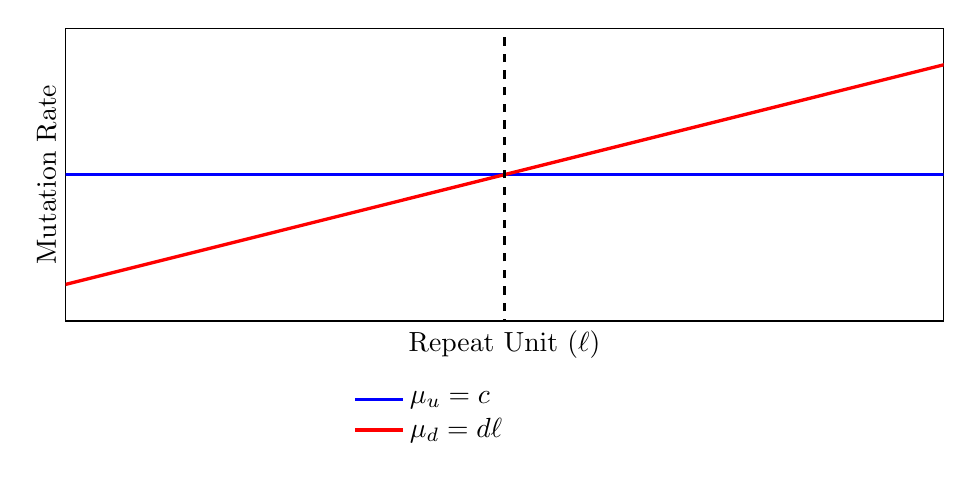
\begin{tikzpicture}
    \begin{axis}[
    width=1.05\linewidth, height=5.3cm,
    ylabel={Mutation Rate}, ymin=0.01, ymax=0.05,
    xlabel={Repeat Unit ($\ell$)}, xmin=6, xmax=18,
    xtick={0, 2, 4, 6, 8, 10, 12, 14, 16, 18, 20, 22, 24},
    samples=100, no markers, enlargelimits=false, legend style={at={(0.5,-0.2)},anchor=north,draw=none},
    legend cell align={left}, domain=0:25, ticks=none
    ]
        \addplot+[very thick]{0.03};
        \addlegendentry{$\mu_u = c$};

        \addplot+[very thick] {0.0025*x};
        \addlegendentry{\vspace*{5em}$\mu_d = d\ell$ \hspace*{5em}};

        \addplot+[very thick, black, dashed, forget plot] coordinates {(12, 0) (12, 0.05)};
    \end{axis}
\end{tikzpicture}} \newline
            \end{column}
        \end{columns}

        \note{
            \footnotesize
            \begin{enumerate}
                \item Third essential question: \ldots
                \item There exists a lot of research toward accurately characterizing microsatellite mutation in
                    humans, but the focus of my project lies with the methodology.
                \item To prove my methods, we want a flexible model with a small number of parameters.
                \item Our first point comes from Ohta and Kimura: Microsatellites mutate up one, down one, or
                    stay the same per generation.
                \item Our second point comes from Kruglyak: Microsatellites mutate differently at different repeat
                    lengths.
                \item The third point comes from Garza: Microsatellites mutate toward some focal length.
                \item This brings us to our model: we have two lines that always intersect each other, using three
                    parameters: $c, u, d$.
            \end{enumerate}
        }
    \end{frame}

    \section{Methodology}\label{sec:m}
	\subsection{Coalescent Simulation}\label{subsec:c}
    \begin{frame}
        \frametitle{How do we simulate evolution?}
        \begin{columns}
            \begin{column}{0.6\textwidth}
                \emph{Answer:} We construct a evolutionary tree! \medskip
                \begin{enumerate}
                    \item Given sample size $n$, parameters $c, u, d$. \medskip
                    \item Construct random tree with $n$ leaves and common ancestor. \medskip
                    \item Randomly choose repeat unit of common ancestor. \medskip
                    \item Mutate children from ancestors until leaves are reached.
                \end{enumerate}
            \end{column}
            \begin{column}{0.4\textwidth}
                \centering{\usetikzlibrary{decorations.pathreplacing}
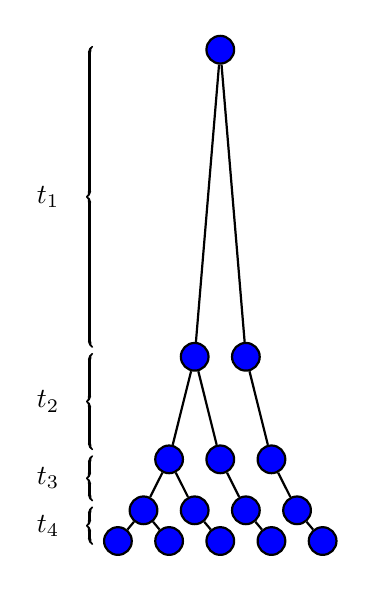
\begin{tikzpicture}[scale=0.65]
    \begin{scope}[auto, every node/.style={draw=black,circle,thick,minimum size=1em,fill=blue}]
        \node (A_1) at (1, 0) {};
        \node (A_2) at (2, 0) {};
        \node (A_3) at (3, 0) {};
        \node (A_4) at (4, 0) {};
        \node (A_5) at (5, 0) {};

        \node (B_1) at (1.5, 0.5*1.2) {};  % N = 5, 5 choose 2 = 10, 5 / 10 = 0.5
        \node (B_2) at (2.5, 0.5*1.2) {};
        \node (B_3) at (3.5, 0.5*1.2) {};
        \node (B_4) at (4.5, 0.5*1.2) {};

        \node (C_1) at (2, 1.33*1.2) {};  % N = 5, 4 choose 2 = 6, 5 / 6 = 0.83
        \node (C_2) at (3, 1.33*1.2) {};
        \node (C_3) at (4, 1.33*1.2) {};

        \node (D_1) at (2.5, 3*1.2) {};  % N = 5, 3 choose 2 = 3, 5 / 3 = 1.66
        \node (D_2) at (3.5, 3*1.2) {};

        \node (E_1) at (3, 8*1.2) {};  % N = 5, 2 choose 2 = 1, 5 = 5
    \end{scope}

    \begin{scope}[every edge/.style={draw=black,thick}]
        \path (A_1) edge (B_1);
        \path (A_2) edge (B_1);
        \path (A_3) edge (B_2);
        \path (A_4) edge (B_3);
        \path (A_5) edge (B_4);

        \path (B_1) edge (C_1);
        \path (B_2) edge (C_1);
        \path (B_3) edge (C_2);
        \path (B_4) edge (C_3);

        \path (C_1) edge (D_1);
        \path (C_2) edge (D_1);
        \path (C_3) edge (D_2);

        \path (D_1) edge (E_1);
        \path (D_2) edge (E_1);
    \end{scope}

    \node (T_A) at (0.5, -0.25) {};
    \node (T_B) at (0.5, 0.6+0.25) {};
    \draw[decoration={calligraphic brace,amplitude=2pt},decorate,line width=1.2pt]
    (T_A) -- node[anchor=east, xshift=-8pt] {$t_4$} (T_B);

    \node (T_B2) at (0.5, 0.6) {};
    \node (T_C) at (0.5, 1.6+0.25) {};
    \draw[decoration={calligraphic brace,amplitude=2pt},decorate,line width=1.2pt]
    (T_B2) -- node[anchor=east, xshift=-8pt] {$t_3$} (T_C);

    \node (T_C2) at (0.5, 1.6) {};
    \node (T_D) at (0.5, 3.6+0.25) {};
    \draw[decoration={calligraphic brace,amplitude=2pt},decorate,line width=1.2pt]
    (T_C2) -- node[anchor=east, xshift=-8pt] {$t_2$} (T_D);

    \node (T_D2) at (0.5, 3.6) {};
    \node (T_E) at (0.5, 9.6+0.25) {};
    \draw[decoration={calligraphic brace,amplitude=2pt},decorate,line width=1.2pt]
    (T_D2) -- node[anchor=east, xshift=-8pt] {$t_1$} (T_E);
\end{tikzpicture}}
            \end{column}
        \end{columns}

        \note{
            \footnotesize
            \begin{enumerate}
                \item
            \end{enumerate}
        }
    \end{frame}

	\subsection{ABC MCMC}\label{subsec:abcmcmc}
    \begin{frame}
        \frametitle{How can we find the best parameters?}
        \begin{columns}
            \begin{column}{0.6\textwidth}
                \begin{itemize}
                    \item \emph{Problem}: Which model parameters are the most likely to generate our observed data?
                        \begin{enumerate}
                            \item How do we compute this likelihood? \smallskip
                            \item How can we maximize this likelihood?
                        \end{enumerate} \bigskip
                    \item \emph{Solution}: ABC -- MCMC (\footnotesize{Approximate Bayesian Computation -- Markov
                        Chain Monte Carlo})
                \end{itemize}
            \end{column}
            \begin{column}{0.4\textwidth}
                \begin{flushleft}
                    \pgfplotsset{compat=1.5}
\pgfmathdeclarefunction{gauss}{2}{%
  \pgfmathparse{1/(#2*sqrt(2*pi))*exp(-((x-#1)^2)/(2*#2^2))}%
}

\begin{tikzpicture}
    \begin{axis}[
    width=1.15\linewidth, height=6.4cm,
    ylabel={Likelihood}, ymax=0.3,
    xlabel={Parameter Value}, xmin=0, xmax=10,
    samples=100, no markers, enlargelimits=false, legend style={at={(0.5,-0.35)},anchor=north},
    domain=0:25, ticks=none
    ]
    \addplot [very thick,blue!50!black] {gauss(5,1.5)};

    \addplot+[very thick, black, dashed] coordinates {(0, 0.26596152) (25, 0.26596152)};
    \end{axis}
\end{tikzpicture}
                \end{flushleft}
            \end{column}
        \end{columns}

        \note{
            \footnotesize
            \begin{enumerate}
                \item
            \end{enumerate}
        }
    \end{frame}

    \begin{frame}
        \frametitle{How do we compute likelihood?}
        \begin{columns}
            \begin{column}{0.6\textwidth}
                \begin{itemize}
                    \item \emph{Problem}: Frequency of exact matches is low. \bigskip
                    \item \emph{Solution}: Count approximate matches instead!
                        \begin{enumerate}
                            \item Quantify difference $\delta$ between observed and generated.
                            \item Run simulation several times.
                            \item Count number of generated samples where $\delta$ is below some threshold.
                        \end{enumerate}
                \end{itemize}
            \end{column}
            \begin{column}{0.4\textwidth}
                \begin{flushleft}
                    \pgfplotsset{compat=1.5}
\pgfmathdeclarefunction{gauss}{2}{%
  \pgfmathparse{1/(#2*sqrt(2*pi))*exp(-((x-#1)^2)/(2*#2^2))}%
}
\pgfmathdeclarefunction{smallergauss}{2}{%
  \pgfmathparse{0.03/(#2*sqrt(2*pi))*exp(-((x-#1)^2)/(2*#2^2))}%
}

\begin{tikzpicture}
    \begin{axis}[
    width=\linewidth, height=6.4cm,
    ylabel={Likelihood}, ymax=0.03,
    xlabel={Parameter Value}, xmin=0, xmax=40,
    samples=100, no markers, enlargelimits=false, legend style={at={(0.5,-0.35)},anchor=north},
    domain=0:40, ticks=none
    ]
    \addplot [very thick,blue!50!black] {smallergauss(20,1.5)};
    \addplot [very thick,red!50!black] {gauss(20,20)};

    \end{axis}
\end{tikzpicture}
                \end{flushleft}
            \end{column}
        \end{columns}

        \note{
            \footnotesize
            \begin{enumerate}
                \item
            \end{enumerate}
        }
    \end{frame}

    \begin{frame}
        \frametitle{How do we maximize likelihood?}
        \begin{columns}
            \begin{column}{0.6\textwidth}
                \begin{itemize}
                    \item \emph{Problem}: Cannot write likelihood function for simulator model. \bigskip
                    \item \emph{Solution}: Use MCMC!
                        \begin{itemize}
                            \item Randomly samples from likelihood distribution (walks).
                            \item Spends longer time in regions of high likelihood.
                            \item Frequency of samples is proportional to likelihood.
                            \item Fit frequency to curve, maximize this curve.
                        \end{itemize}
                \end{itemize}
            \end{column}
            \begin{column}{0.4\textwidth}
                \begin{flushleft}
                    \pgfplotsset{compat=1.5}
\pgfmathdeclarefunction{gauss}{2}{%
  \pgfmathparse{1/(#2*sqrt(2*pi))*exp(-((x-#1)^2)/(2*#2^2))}%
}

\begin{tikzpicture}
    \begin{axis}[
    width=1.15\linewidth, height=6.4cm,
    ylabel={Likelihood}, ymax=0.3,
    xlabel={Parameter}, xmin=0, xmax=10,
    samples=100, no markers, enlargelimits=false, legend style={at={(0.5,-0.35)},anchor=north},
    domain=0:25, ticks=none
    ]
    \addplot [very thick,blue!50!black] {gauss(5,1.5)};
    \addplot+[very thick, black, dashed] coordinates {(2.5, 0.06631809) (2.5, 0.16131382) (3.5, 0.16131382)};
    \addplot+[very thick, black, dashed] coordinates {(3.5, 0.16131382) (3.5, 0.25158882) (4.5, 0.25158882)};
    \addplot+[very thick, red, dashed] coordinates {(4.5, 0.25158882) (4.0, 0.25158882) (4.0, 0.21296534)};

    \end{axis}
\end{tikzpicture}
                \end{flushleft}
            \end{column}
        \end{columns}

        \note{
            \footnotesize
            \begin{enumerate}
                \item
            \end{enumerate}
        }
    \end{frame}

    \section{Results}\label{sec:r}
    \subsection{Posterior Distribution}\label{subsec:pd}
    \begin{frame}
        \frametitle{What are our results?}

        \scriptsize{
            \begin{align*}
                \text{Hyperparameters}: \mathit{I} &= 50000, \mathit{SPP} = 100, \tau = 0.5, f = 100, n = 50, \\
                g_d &= N(1.65, 0.1), g_c = N(0.002, 0.0002), g_u = N(0.01, 0.002) \\
                \mathcal{D} &= \text{Columbian Populace}
            \end{align*}
        }

        \note{
            \footnotesize
            \begin{enumerate}
                \item
            \end{enumerate}
        }
    \end{frame}

    \subsection{Trace Plot}\label{subsec:tp}
    \begin{frame}
        \frametitle{How do we know if this is correct?}

        \note{
            \footnotesize
            \begin{enumerate}
                \item
            \end{enumerate}
        }
    \end{frame}

    \section{Conclusion}\label{sec:c}
    \begin{frame}
        \frametitle{Conclusion}

        \begin{enumerate}
            \item
        \end{enumerate}
    \end{frame}

    \begin{frame}
        \frametitle{Acknowledgments}
        \begin{itemize}
            \item Dr. Floyd Reed \bigskip
            \item Reed Lab \bigskip
            \item Undergraduate Showcase \bigskip
            \item UHM Mathematical Biology Committee \bigskip
            \item The Audience
        \end{itemize}
    \end{frame}

    \begin{frame}
        \frametitle{References}
        \tiny
        \bibliographystyle{abbrv}
        \bibliography{include/references}
    \end{frame}

    \begin{frame}
        \centering{\huge{Questions? :-)}}
    \end{frame}

\end{document}